% for sublime text 3
%!TEX root = diss.tex

\chapter{Coherence Modeling}
\label{ch:coherence}

Local coherence modeling is a crucial task for natural language processing with varying specifications over the years. 
This chapter gives related linguistic definitions, which are related to the task that is tackled in this thesis. 


\section{Problem Definition}
\label{sec:coh-def}

In this thesis, we tackle the problem of local coherence modeling. 
The popular definition of this task is to model how sentences in a text are related one another. 
This task has been the focus of the majority work in text processing (see Chapter \ref{ch:rel-work}). 
Variations of the task consider different types of relations, such as rhetorical \cite{hovyeduard89} or lexical \cite{morris91}, between different spans of texts, such as clauses \cite{strube.col98} or sentence \cite{halliday76}, in various text types, such as dialogue \cite{wangxinhao13} or monologue \cite{barzilay08}. 
Here we give a formal definition of this problem, which will be used in the following chapters of this thesis. 

\subsection{Formal Modeling}

In order to provide a formal definition of the task, i.e.\ local coherence modeling in texts, we first need to give a definition of what we refer to as a text. 
In this thesis, the word text refers to formal written and monologue sequence of sentences that transmit a meaning as a whole.  
We assume that a text consists of more than one sentence. 

\begin{definition}
Text $T$ is a sequence of finite number of sentences $[s_0, s_1, s_2, ..., s_n]$ where the number of sentences is greater than 1, $n>0$.   
\end{definition}

Each sentence in the above definition of a text is a list of words that form a sentence structure. 

\begin{definition}
Sentence $s_i$ is a sequence of words $[w_0, w_1, w_2, ... , w_n]$ that form a sentence structure in the language. 
\end{definition}

An underlying assumption in research on text processing is that a text is more than the sum of its sentences. 
It is not sufficient to collect an arbitrary sequence of sentences in order to obtain a text. 
Sentences in a text are supposed to be related to one another to make a whole. 

\begin{definition}
A relationship function $R(s_i,s_j)$ indicates whether two given sentences in a text are related. 
The domain of this function is sentences in a text and its range is a binary value $
\lbrace 0,1\rbrace$. 
\end{definition} 

Having the above definition, relationships across all sentences in a text can be represented by a set $P$ containing relationships between any pairs of sentences in the text. 

\begin{definition}
Let $r_{ij}= R(s_i,s_j)$ indicates the relationship between a sentence pair $(s_i,s_j)$ in a text $T$, the set $P$ contains all $r_{ij}$ for any pair of sentences in $T$.
\end{definition}  

Although we define $P$ as a set but it can be partially structured, e.g.\ when sentence $s_i$ has to proceed sentence $s_j$ in a text. 


While some texts can be simply recognized as coherent or incoherent, often it is a matter of degree \cite{halliday76}. 
A text can be less coherent when compared to one text, but more coherent when compared to another. 
As such, since the notion of coherence is relative, coherence assessment is better represented as a ranking problem. 
Given a pair of texts, a model ideally ranks them with respect to their coherence.
In order to rank texts with respect to their coherence, we need to capture patterns that frequently occur in well-written texts, and rarely in less coherent ones.  
Coherence patterns are template of relationships among sentences in texts, such that their frequencies assist to distinguish coherent texts from incoherent ones. 

\begin{definition}
A coherence pattern is a subset of relations $p \subseteq P$ occurring among sentences of a text.   
\end{definition}

We define a function to model how coherence patterns are extracted from a corpus of texts. 

\begin{definition}
Given a corpus $C$ which includes texts with different degrees of coherence, a pattern mining method $M$ extracts all subsets of relations that occur in texts in $C$. 
\end{definition} 

The output of the pattern mining process on a corpus of texts is a set of coherence patterns. 
The coherence of a text can be modeled by a vector of frequencies of these patterns in the text. 

\begin{definition}
Let $P=\lbrace p_0,p_1,p_2,...,p_m \rbrace$ be a set of extracted patterns from a corpus of texts $C$, the perceived coherence of each text $T$ is represented by a vector $\phi = <f_0, f_1, f_2,...,f_m>$, where $f_k$ is the frequency of pattern $p_k$ in text $T$. 
\end{definition}

Having vector representations of coherence lets us to employ machine learning models to rank texts. 
In Chapter \ref{ch:rel-work}, we describe different approaches to modeling relationships between a pair of sentences, i.e.\ $R(s_i,s_j)$, and how they represent the set of all relations in a text $P$.  
There, we also review how method $M$ is derived by different computational models. 
We employ a powerful representation method from the literature and develop our approach for extracting coherence patterns in Chapter \ref{ch:coh-patterns}. 
We further improve the predictive power of coherence patterns by a new approach to relationship representation among sentences $P$ in Chapter \ref{ch:lex-graph}. 

\section{The Linguistics of Coherence}

The aforementioned formal definition of the problem is sufficient for the research in this thesis to develop a representation of cohesive relations in a text, and extract coherence patterns. 
However, since coherence is a semantic property of a text, the definition needs to be related with linguistic properties of a text. 

Our aim is to develop an approach which provides a representation of the coherence of a text. 
Therefore we need to understand what aspects in sentences serve to relate sentences and how coherence patterns are modeled in linguistics of coherence. 
Therefore, we explain related linguistic properties that are required to complete our definition. 


\subsection{Text}

The first definition in our formal model of coherence is about text. 
In linguistic research the word ``text'' is used to refer to any passage, spoken or written, of whatever length that forms a unified whole \cite{halliday76}. 
In this thesis, we follow other coherence models \cite{barzilay08,guinaudeau13} and use the word ``text'' to denote a merely monologue written passage, which is more than one sentence.
One sentence texts, of course, do exist, like public notices, proverbs and advertising slogans and the like. 
An a sample text in Example \ref{ex:coh-one-sent-text}\footnote{Taken from \url{https://www.engvid.com/english-resource/50-common-proverbs-sayings/}, accessed 1 June 2018.}: 

\begin{examples}
    \label{ex:coh-one-sent-text}
    A journey of a thousand miles begins with a single step.
\end{examples}

However, due to texts consisting of one sentence only are fairly rare, we assume texts contains several sentences.  
We also assume that texts are written in a formal language, in contrast to informal like tweets\footnote{A post made on the social media application Twitter}. 

\subsection{Coherence}

Coherence is a crucial factor of a well-written text. 
It makes the text distinguishable from an unrelated sequence of sentences. 
We follow \newcite{stede12} and define coherence as a property of a text that is designed around a common topic. 
A coherent text discusses a sequence of topics in a structured way that a reader can recognize and relate to one another, and collectively render the text as a unified whole. 
Each topic is tending to occupy a (topical) segment of the text \cite{hearst97}. 
Coherence is defined based on the relations and structures of topical segments in a text. 
This structure is sometimes referred to as global, since it is coarse-grained and spans the entire text \cite{elsner07}. 
\newcite{lautamatti78} defines the term topic as what the sentence is about and the term comment as information about the topic.  
In general, however, defining the notion of topic, and recognizing topics and the boundaries between  text segments corresponding to them are not straight forward \cite{stede12}. 
We discuss some computational topical coherence model in Chapter \ref{ch:rel-work}. 


\subsection{Local Coherence}

From the linguistic viewpoint, a coherent text employs linguistic devices, more-readily identifiable linguistic signals, to relate sentences of a text to each other. 
These devices signal readers to interpret each sentence considering its relations with other linked sentences \cite{vandijk77}. 
Therefore, understanding the text implies uncovering these relationships.  
The way that linguistic devices are used to relate sentences in a text is known as local coherence. 
In some literature in text linguistics \cite{halliday76}, this phenomena is referred to as cohesion.   
\newcite{stoddard91} (chapter 2) argues that these two are not distinguishable and can be used interchangeably. 
\newcite{stede12} states that signals of local coherence serve as indicators of topic continuity, consequently the absent of a surface relation is a sign of topic shift. 
Since the research in this thesis is about modeling local coherence, henceforth in this thesis it is referred to as coherence modeling, unless this is not clear from the context. 

Prominent cohesive devices can be grouped in grammatical and lexical relations between elements of sentences \cite{halliday76}. 
Grammatical relations are reference, substitution, ellipsis and conjunctions. 
Lexical relations include any lexical-semantic relation, such as repetition, synonym, antonym, and the like, between words of sentences. 
Reference cohesive devices are also known as entity-based relations, with the intuition that related sentences in a text keep referring to the same named entity. 
We follow \newcite{barzilay05a} and \newcite{elsner10} regrading entity definition.  

\begin{definition}
    An entity is as a person, an object or abstraction that exists (or could exist) external world to a text. 
\end{definition}

An entity can be referred to in different ways by various referral expressions, or mentions. 

\begin{definition}
	Pieces of a text that are used to refer to an entity are called \emph{mentions}. 
\end{definition}

Having these definitions, one way of representing an entity is to group all mentions that refer to that entity. 
The task of identifying mentions that refer to the same entity is known as coreference resolution task.  
The goal of this task is to cluster mentions of a text based on entities that they are referring to.  

\begin{definition}
	The task of detecting all mentions in a text and clustering all mentions that refer to same entities is called \emph{coreference resolution}. 
\end{definition}

Each cluster, which can be imagined as a bucket containing all referent mentions, represent an entity. 

The sample text in Example \ref{ex:coh-ref}\footnote{Taken from \url{https://web.stanford.edu/class/archive/cs/cs224n/cs224n.1162/handouts/cs224n-lecture11-coreference-6up.pdf}, on June 2 2018.} shows how entity-based relation link sentences. 

\begin{examples}
	\label{ex:coh-ref}
	\textbf{Mr.\ Obama} visited the city. \\
	\textbf{The president} talked about Milwaukee’s economy. \\
	\textbf{He} mentioned new jobs. \\
\end{examples} 

One of the popular entity-based frameworks for local coherence modeling is Centering Theory \cite{grosz95}. 
The main hypothesis of this theory is the center that at any given point in a text is most salient entity.  
The center captures the focus of attention in the reader mind \cite{grosz95}.
Centering Theory accounts of the process of flowing the center in a text. 
The original centering theory (for English texts) see the grammatical role as the most important linguistic sign of the text center. 
Specifically, the grammatical subject is taken the default position for the text center. 
Depending on the configuration of grammatical roles in adjacent sentence, \newcite{brennan87} define four different types of transitions for the text center. 
These transitions capture the smoothness of the center move from one sentence to another. 
When a latter sentence focuses on the topic, i.e.\ center, transition is Continue, the other types involve topic shift: Retain, Smooth Shift, and Rough Shift. 
Centering has been applied directly in models of coherence \cite{karamanis04a}.  
However, since it requires human annotations for transitions between sentences, other models employ the basic Centering principles as soft constraints or features in a probabilistic framework such as the Entity Grid \newcite{barzilay05a,barzilay08}, which we discuss in more detail in Chapter \ref{ch:rel-work}.

Further research shows that grammatical role information are far less predictive for tracking the text center in German, as a free word order language \cite{strube.acl96}. 
Instead the functional information structure \cite{danes74} are considered. 
This structure captures flows between given information versus new information in a text. 
Some information in a sentence is known or old, because of it is discussed by preceding sentences of the sentence, and some information are new. 
The functional information structure is explained by \newcite{halliday76} as theme-rheme relations in a text. 
Theme can be taken as given information, as a point of the text departure, and rheme is (almost) similar to new information, as clarity information in the theme. 
While theme conveys information that is initially introduced in discourse, rheme presents specific 
information regarding the theme. 
As the theme-rheme movement continues through a text, ideas in the text are expected to flow along smoothly and are easier for the reader to understand. 
Thematic relations between sentences in texts reveal some patterns \cite{danes74}, which are called  coherence patterns.
In Chapter \ref{ch:coh-patterns}, where we define our coherence patterns, we give more explanation about functional information structure \cite{danes74} in texts. 

The other perspective of local coherence is lexical cohesion, which cohesive effect based on lexical-semantic relations between words. 
An advantage of lexical cohesion, on contrary to entity-based models, is that it requires no annotation at all; they are accessible directly from the text. 
The insight of local coherence on the grounds of lexical relations is that content words in a text do not occur independently of one another, but bear semantic similarity because of common topic. 
A form of lexical cohesion is reiteration, which involves different type of lexical relations such as repeating a word, using a synonym of a word, employing a superordinate word, and using a general word. 
Example \ref{ex:coh-lex} is taken from \cite{halliday76} to illustrate these relations:

\begin{examples}
	\label{ex:coh-lex}
	(a) Repetition: There was a large \textbf{mushroom} growing near her, about the same height as herself; and when she had looked under it, it occurred to her that she might as well look and see what was on the top of it.\\
	She stretched herself up on tiptoe, and peeped over the edge of the \textbf{mushroom}, ... 

	(b) Synonymy: Accordingly ... I took leave, turned to the \textbf{ascent} of the peak. \\
	The \textbf{climb} is perfectly easy. 

	(c) Superordinate: Henry's bought himself a new \textbf{Jaguar}. \\
	He practically lives in the \textbf{car}. 

\end{examples} 

In (c) the word ``car'' is a superordinate, any word whose meaning includes that of the earlier one, of ``Jaguar'', as vehicle is a superordinate of the car, spoon of teaspoon, and the like. 
The boundary between the reiteration type of lexical cohesion and reference type in grammatical relations, i.e.\ entity-based relations, is by no means clearcut\footnote{However, properly speaking, reference is irrelevant to lexical cohesion. As we discuss later lexical cohesion relationship between two items does not need to imply a coreferent relationship.} \cite{halliday76}. 
This can slightly clarify the reason that for purposes of the research in this thesis local coherence and cohesion are largely synonymous.

It is not necessary for two lexical occurrences to be coreferent, however, in order to for them to be cohesive. 
Consider Example \ref{ex:coh-nonref} from \newcite{halliday76}(p.~282). 
In (a) word ``boy'' and  word ``boys'' are not coreferent, however, their semantic relationship serves to link the sentences. 
This relationship is not in any way dependent on the presence of other items; it is not the wriggling that provides the context, as (b) shows. 

\begin{examples}
	\label{ex:coh-nonref}
	Why does this little boy have to wriggle all the time? \\
	(a) Good boys don't wriggle. \\
	(b) Boys should be kept out of here. \\
\end{examples} 

This leads to a systematic relationship between a pair of words, that is because the words are frequently occur in similar text context. 
For instance, words ``boy'' and ``girls'' in Example \ref{ex:coh-collocation} \cite{halliday76}(p.~285) relate the sentence, although they are not coreferent, or even synonym. 

\begin{examples}
	\label{ex:coh-collocation}
	Why does this little boy have to wriggle all the time? \\
	Girls don't wriggle. 
\end{examples}

In summary, there is a local coherence relation between any pair of lexical items that stand to each other in some lexical-semantic relations. 
This includes any type of relations, such as relations between word pairs shown in Example \ref{ex:coh-word-pairs} \cite{halliday76} (p.~285). 

\begin{examples}
	\label{ex:coh-word-pairs}
	rail ... road \\
	car ... brake \\
	try ... succeed \\
	walk ... drive \\
	Tuesday ... Thursday \\
	like ... hate \\
	red ... green 
\end{examples}

For textual purposes, it is (almost) sufficient to know that a pair of words are in a relationship, rather than the type of relation \cite{halliday76} (p. 285).  
\newcite{hoey91} examine how lexical cohesive elements make a text organized, and contribute to local coherence. 
He shows that relations between semantically related words in a text can make patterns in texts. 
In Chapter \ref{ch:rel-work}, we survey some related computational models of lexical cohesion in texts. 

% % One of the basic approaches to lexical cohesion is \emph{Cohesion in English} \cite{halliday76}. 
% % Halliday and Hasan’s model of lexical cohesion is based on a division of the various lexical cohesive devices into two main categories: reiteration and collocation. 
% % Reiteration includes the repetition of the same word (mushroom – mushroom), the use of a synonym (sword – brand), the use of a superordinate (Jaguar – car), and the use of a general word (We all kept quiet. That seemed the best move.). 
% % All these devices have the function of reiterating the previous item, either in an identical or somewhat modified form, and this is the basis for the creation of a cohesive tie between the items.
% % Often the tie is strengthened by the fact that the items are co-referential, but as \newcite{halliday76} \textbf{Halliday and Hasan (1976: 282– 283)} note, this is not required for two items to be cohesive; even without co-referentiality, two occurrences of an item in a text will constitute a tie, as in the following example .
% % There’s a boy climbing that tree. Most boys do!

% % According to Halliday and Hasan, collocation is ``cohesion that is achieved through the association of lexical items that regularly co-occur'' (Halliday \& Hasan 1976: 284). 
% % This general definition of collocation may seem a little vague, but they do try to clarify it: the association is achieved when the lexical items have a tendency to appear in similar lexical environments or when they are related lexicosemantically. 
% % For example, boy and girl are cohesive because they have opposite meanings, but laugh and joke, and boat and row are also cohesive, although they are not systematically related, only ``typically associated with one another'' (Halliday \& Hasan 1976: 284–286).

% % What differentiates between collocation in the lexicographic sense, on the one hand, and in the cohesive sense, on the other, is the proximity of the items. In lexicography, collocation refers to adjacent items: the item investigated is called the node, and a restricted number of items (typically from four to six) positioned on either side of the node are its collocates. But since cohesion refers to connections between longer stretches of a text (clauses and sentences), items that are regarded as being related by collocation in the cohesive sense cannot be adjacent in that text. We can here reconsider Firth’s example of night and dark: if they occur next to each other, they are an instance of lexicographic col- location, but if they are separated by a longer stretch of text, their relationship ties together the clauses or the sentences in which they occur and they can be regarded as an instance of cohesive collocation.

% Segmentation into a linear sequence of topically coherence segments generally assumes that the topic of a segment will differ from that of adjacent segments. It is also assumed that topic constrains lexical choice. either of all words of a segment or just its content words (i.e., excluding stop-words).
% Topic relation is based on either semantic-relatedness or topic models. 
% The elements for making connections are either sentences or a pseudo-sentences (i.e., fixed length string) whose relevant elements may be all the words or just content words .
% All semantic-relatedness approaches to topic segmentation involve (1) a metric for assessing the semantic relatedness of terms withing proposed segments (2) a locality that specifies which units within a text are assessed for semantic relatedness, (3) a threshold for deciding how low relatedness can drop before it signals a shift to another segment.

% % This type of relationship is the most problematic, especially from a knowledge representation point of view. Such collocation relationships exist between words that tend to occur in similar lexical environments. Words tend to occur in similar lexical environments because they describe things that tend to occur in similar situations or contexts in the world. Hence, context-specific examples such as {post office, service, stamps, pay, leave} are included in the class.

% According to Morris and Hirst (1991), lexical cohesion is the result of chains of related words that contribute to the continuity of lexical meaning. 



\subsection{Coherence Patterns}
\textbf{stodarrd a and some part from danes}

An increasing number of researchers and practitioners in natural language processing face the prospect of having to work with entire texts, rather than individual sentences. 
While it is clear that text must have useful structure, its nature is less clear, making it more difficult to exploit in applications \cite{webber12a}. 
A text commonly comprises a sequences of sentences. 
Within a text, the patterns formed by its sentences mean that the whole conveys more than the sum of its separate parts. 
Text structures are the patterns that one sees in multi-sentence texts \cite{webber12a}. 
Recognizing these patterns in terms of the elements that compose them is essential to correctly deriving and interpreting information in the text. 
The elements may be topic, each  about a set entities and what is being said about them.
Texts can be structured by its topics, each comprising a set of entities and a limited range of things being said about them. 
Patterns of coherence relations can also be characteristic of particularly types of text, and therefore be of value in assessing the quality of automatically generated text. 

The concept of coherence pattern is linguistically derived from the texture of texts. 
\newcite{stoddard91} defines a text as ``a phenomenon of seemingly infinite complexity because of its synergistic nature'' where elements of a text are supposed to corporate together for an enhanced effect. 
It is synergism that makes texts more than sequential words and sentences. 
The dynamic of synergism, which is because of its multidimensionality, is beyond the linear, sequential structure of texts. 
One cause of the multidimensionality of synergism is a global component which can be referred to as ``texture" that is 
the quality created by the combination of the different elements in a text. 
Indeed, one of the preliminary principles of texture is coherence, which is a type of unifying device which we construct consciously or unconsciously, as we process texts \cite{stoddard91,halliday76}.

From \newcite{stoddard91}'s perspective, the texture of texts is interpretable by means of elements that are common in all texts and those that differentiate texts. 
These elements are referred to as patterns of coherence. 
\newcite{stoddard91} believes that the texture property of texts manifests itself in patterns of coherence in written texts. 
It is worth noting that texture, in one sense, involve the quality of depth, which may range from minimal (approximating ``flatness") to maximal, or at any level in between. 
In other words, patterns of coherence can be as basic as the linear order of elements of a text or be more complicated. 
\newcite{stoddard91} describes the texture of texts as a composite of patterns -- storyline patterns, rhetorical patterns, linguistic patterns and so on -- which when overlaid to create the totality of a text creates variant textures which are like ``fingerprint'' of a text. 
In this sense, the texture of texts is more closely to ``style'', which are certainly related \cite{sedelow66,stoddard91} to local coherence \cite{barzilay08}. 

Other linguistics also relate what we call coherence patterns to the texture or the nature of texts. 
\newcite{halliday76} claim that ``linguistic patterns  [...] embody, and at the same time impose structure on our experience of the environment ..."
Because of this, they suggest, patterns help us to understand a text as coherent and consistent with our knowledge, experience, and environment. 

One factor that must be considered in describing coherence patterns as input to texture is the likelihood of a pattern occurring over large stretch of a text \newcite{stoddard91} . 
The unity of texts happens because readers perceive the interactiveness of ``text components''. 
Because these appear to have a degree of consistency across all texts, they should be identifiable as texture-forming mechanisms.
Moreover, this would be easier for readers to smoothly process a text in that the patterns of interactiveness among components are familiar to the reader.  

\newcite{stoddard91} illustrated the patterns of cohesion and the way that they interact graphically for a few texts. 
The term of ``networks of cohesion" proposed by \newcite{halliday76} is anaphoric for this graphical illustration. 
The result of text analysis in \newcite{stoddard91} showed that the local coherence creates pattern, and she suggests to unify a text by means of coherence network patterns that span varying lengths of text passage. 
The importance of the results lies in the fact that typologies (i.e. graphical structure) and counting, when supplemented with other kinds of analysis, give us a better understanding of local coherence as it contributes to the texture of a text. 

The fact that cohesive patterns occur in texts and the fact that cohesiveness is relative in texts provide useful validation of our intuition: coherent texts reveal some regularities in their structure that can be encoded by the frequency of coherence patterns. 

Another linguistic research related to coherence patterns is done by \newcite{danes74a}. 
She describes the structure of texts by the concept  of ``thematization" that has been also noticed by \newcite{halliday76} as ``information focus" or given-new information. 
\newcite{halliday67} summarize in the this way that ``given information" has been talked about in a text and ``new information" is been mentioning now.  
Similarly, theme, from the \newcite{danes74a}'s point of view, is ``the point of departure" where the text flows from a topic (``given information") towards another topic (``old information"). 
In simple words, theme can be realized as ``given information" and rhyme is ``new information" and ``thematization"  is about  patterns of transitions between themes and rhymes in a text. 

The contextual determination of givenness is far from being a simple phenomena \cite{danes74a}. 
Tentatively, some information that is mentioned directly or indirectly in a text can be interpreted as given information. 
\newcite{danes17} explains that ``given information" can be realized either directly with an identical wording or , indirectly, with a synonymous expression, or with a paraphrase. 
The indirect mentioning is based on semantic inference. 
For instance, the expression ``illness" occurring in a sentence might convey a piece of given information if in one of its preceding sentences ``disease" has been somehow mentioned. 
In contrary, the new information either is not mentioned in its proceeding context or is related to a given information. 
This phenomena is known as the relation between ``theme'' and ``Rhyme" in \newcite{danes74a} as is shown by  $T \rightarrow R$. 
This illustrates that flow of information is from ``given information" (or ``theme") to ``new information" (or ``rhyme").
\newcite{danes74a} believes that the inquiry into the thematic organization of the text is closely connected with the investigation of the so-called ``text coherence" or ``text connectivity" .
She analyzes Czech scientific and other professional texts, as well as some tentative soundings in the area of German and English language materials.
She has ascertained  three major types of organizational patterns in examined texts, represented in Table \ref{Table:danesh_coherence_patterns}. 


\begin{table}
\centering
\begin{tabular}{c|c}
Pattern ID & Pattern \\\hline
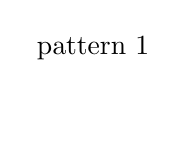
\begin{tikzpicture}
\node [] (n0)  at (0.0,0.0) {};
\node [] (n1)  at (0.0,1.0) {pattern 1}; 
\end{tikzpicture} 
&
\begin{tikzpicture}
\node [] (n1)  at (0.0,2.0) {$T_1 \rightarrow R_1$}; 
\node [] (n2)  at (1.8,1.0) {$T_2 (= R_1) \rightarrow R_3$};
\node [] (n3)  at (4.2,0.0) {$T_3 (= R_2) \rightarrow R_4$}; 

\draw[->] (0.5,1.7) -- (0.5,1.3);
\draw[->] (3.0,0.7) -- (3.0,0.3);


\end{tikzpicture}

\\\hline

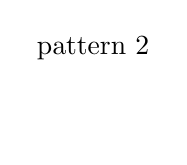
\begin{tikzpicture}
\node [] (n0)  at (0.0,0.0) {};
\node [] (n1)  at (0.0,1.0) {pattern 2}; 
\end{tikzpicture} 
 &
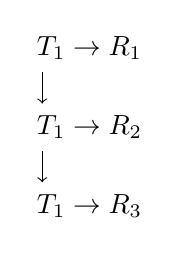
\begin{tikzpicture}
\node [] (n1)  at (0.0,2.0) {$T_1 \rightarrow R_1$}; 
\node [] (n2)  at (0.0,1.0) {$T_1 \rightarrow R_2$};
\node [] (n3)  at (0.0,0.0) {$T_1 \rightarrow R_3$}; 

\draw[->] (-0.6,1.7) -- (-0.6,1.3);
\draw[->] (-0.6,0.7) -- (-0.6,0.3);
\end{tikzpicture}

\\\hline
\begin{tikzpicture}
\node [] (n0)  at (0.0,0.0) {};
\node [] (n1)  at (0.0,2.0) {pattern 3}; 
\end{tikzpicture} 
&
\begin{tikzpicture}
\node [] (n0)  at (2.2,4.0) {$[T]$}; 
\node [] (n1)  at (0.0,3.0) {$T_1 \rightarrow R_1$}; 
\node [] (n2)  at (1.8,2.0) {$T_2 \rightarrow R_2$};
\node [] (n3)  at (4.2,1.0) {$T_3  \rightarrow R_3$}; 

\draw[->] (n0.south) -- (-0.5,3.3);
\draw[->] (n0.south) -- (1.3,2.3);
\draw[->] (n0.south) -- (3.5,1.3);
\end{tikzpicture}

\\\hline

\begin{tikzpicture}
\node [] (n0)  at (0.0,0.0) {};
\node [] (n1)  at (0.0,2.0) {pattern 4}; 
\end{tikzpicture} 
&
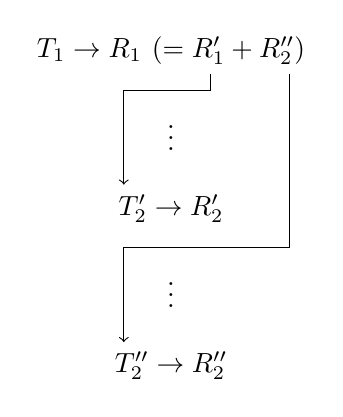
\begin{tikzpicture}
\node [] (n0)  at (0.0,4.0) {$T_1 \rightarrow R_1\textit{ }( = R_1^\prime + R_2^{\prime\prime} )$}; 

\node [] (d0)  at (0.0,3) {$\vdots$}; 

\node [] (n1)  at (0.0,2) {$T_2^\prime \rightarrow R_2^\prime$}; 


\node [] (d0)  at (0.0,1) {$\vdots$}; 


\node [] (n2)  at (0.0,0.0) {$T_2^{\prime\prime} \rightarrow R_2^{\prime\prime}$};

\draw [->] (0.5, 3.7) -- (0.5, 3.5) -- (-0.6, 3.5) -- (-0.6, 2.3);

\draw [->] (1.5, 3.7) -- (1.5, 1.5) -- (-0.6, 1.5) -- (-0.6, 0.3);

\end{tikzpicture}

\end{tabular}
\caption{In the notation used by (?), the horizontal arrow indicates a transition in an utterance, while the vertical one indicates the the contextual connection within of utterances.}
\label{Table:danesh_coherence_patterns}
\end{table}


\newcite{danes74a} interprets the patterns as follows:

\begin{itemize}
\item Pattern 1: A linear transition pattern between themes and rhymes. 
In this pattern, each utterance takes the rhyme presented in the preceding context of the utterance as a given information and transfers it to a new information or a new rhyme. 
In other words, each R (i.e. a new information) becomes the T (i.e. a given information) of the next utterance. 


\item Pattern 2: This pattern depicts a constant theme that continues across utterances. 
One and the same theme appears in a series of utterances. 
Each utterance, however, presents new information about the theme. 


\item Pattern 3: In this pattern $[T]$ indicates a hypertheme that is a global theme of a paragraph or even other text sections. 
 Pattern shows that different utterances can be connected because the themes, or the given information,  of utterances are semantically connected to a hypertheme. 

 \item Pattern 4: 
 \newcite{danes74a} expresses that different combination of these patterns can be employed in different texts. 
 Some of such combinations are so frequent that can be taken as special type of theme-rhyme transition of a higher order. 
  \newcite{danes74a} finds Pattern 4 as one of the most important of such patterns, where an utterance presents two (which can in potential several) rhymes, $R^\prime$ and $R^{\prime\prime}$ , in connection with a given theme. 
  First $R^{\prime}$ expounded and after its progression has been finished, $R^{\prime\prime}$ becomes the theme of another transition. 
  Transitions in between for extending each rhyme follows its own pattern. 
\end{itemize}

\newcite{danes74a} brings this point to the attention that one of the important properties of these patterns is omitting links in these patterns.  
For example, in Pattern 1 there is no link between the earliest and latest utterance. 
Those are connected because there is an intermediate utterance that makes transitions between themes and rhymes smoother. 
In contrast, all utterances in Pattern 3  are linked to each other because they all have $T_1$ as a shared given information. 

\section{Evaluation}
\label{sec:coh-eval}

The goal of the research in this thesis is to provide an approach to coherence modeling and compare it with other models. 
To do so, it is essential to have a method to evaluate the performance of coherence models. 
In this section, we complete the definition of the problem, with which the research in this thesis is tackling, by describing the evaluation method we use for assessing the quality of coherence models. 
Other related approaches for evaluating coherence models are discussed in Chapter \ref{ch:rel-work}. 

\subsection{Intrinsic vs. Extrinsic}

Intrinsic and extrinsic are two types of evaluations methodologies \cite{}. 
In an intrinsic evaluation, system output is directly evaluated in terms of a set of norms or predefined criteria about the desired functionality of the system itself. 
In an extrinsic evaluation, system output is assessed in its impact on a task external to the system itself. 

Some research papers on local coherence modeling use intrinsic evaluation approaches such as sentence ordering \cite{karamanis04a,barzilay04} (see Chapter \ref{ch:rel-work} for a review of other tasks).  
This evaluation method is primarily designed to model violations of restrictions in centering theory \newcite{karamanis04a}. 
The goal is that a coherence model should ideally rank the original order of sentences in a text higher than any permutation of sentences. 

Extrinsic approaches take the coherence of a text as a factor for the quality of the text, given the definition of coherence: What distinguishes a well-written text from others. 
Readability assessment \cite{pitler08} is an example of these approaches. 
In this task, a coherence model is involved with a readability assessment system, which consider other aspect of text quality such as sentence complexity and the like, to evaluate the influence of the coherence model on the end performance of the readability assessment system. 
The insight of this task is that coherent texts are less complex than other ones, therefore they are easy to understand \cite{pitler08}. 

In the this thesis we follow extrinsic evaluation methods: the readability assessment task (see experiments in Chapter \ref{ch:coh-patterns} and Chapter \ref{ch:lex-graph}), and the automatic text summarization task \ref{ch:coh-patterns}. 

\subsection{Ranking as Classification} 

Coherence is not a binary property of a text that either exists or not. 
Rather it is a comparative attribute of texts, whether a text is more coherent than the other one. 
Even for humans it can be ambiguous to decide if a text is coherent or not, however they can rank texts with respect to the coherence property of texts \cite{halliday76}.   

From the computational point of view, the core of the evaluation method in this thesis is a pairwise ranking task: Given a pair of texts, which one is more coherent. 
To be machine learning convenient, the pairwise ranking task is recast as a classification task, where each text pair is associated with a label. 
The value of the label represents which text in the pair should be ranked higher, we use $+1$ where the first text is more coherent, and $-1$ otherwise. 
This binary classification task can be solved by a machine learning approach, such as the Support Vector Machine method \cite{}, for supervised coherence models, like our models in this thesis. 
The details of experimental setups for machine learning models are explained in Chapter \ref{ch:coh-patterns} and Chapter \ref{ch:lex-graph}.  

\subsection{Evaluation Metrics}

In order to perform a quantitative analysis on the predicted labels by a coherence model, we employ the accuracy metric. 
It measures how often a coherence model makes a correct decision. 
A decision is correct if the label predicted by a model for a text pair is identical with the label that is assigned by human judges. 











